% Author: Izaak Neutelings (July 2018)
\documentclass[border=3pt,tikz]{standalone}
\usepackage{amsmath}
\usepackage{tikz}
\usepackage{physics}
\usetikzlibrary{intersections}
\usetikzlibrary{decorations.markings}
\usetikzlibrary{angles,quotes} % for pic
\tikzset{>=latex} % for LaTeX arrow head
\usepackage{xcolor}
\colorlet{Ecol}{orange!90!black}
\colorlet{EcolFL}{orange!80!black}
\colorlet{FCol}{red!60!black}
%\colorlet{charge+}{blue!80!white}
\colorlet{veccol}{green!45!black}
\tikzstyle{charge+}=[thin,top color=red!50,bottom color=red!90!black,shading angle=20]
\tikzstyle{charge-}=[thin,top color=blue!50,bottom color=blue!80,shading angle=20]
\tikzstyle{charge0}=[very thin,top color=green!80!black!50,bottom color=green!80!black,shading angle=20]
%\tikzstyle{charge+}=[thin,ball color=blue!60,shading angle=-10]
%\tikzstyle{charge-}=[thin,ball color=red!85,shading angle=-10]
%\tikzstyle{charge0}=[thin,ball color=green!80!black!80,shading angle=-10]
\tikzstyle{O}=[top color=red!60,bottom color=red!90!black,shading angle=10]
\tikzstyle{H}=[top color=white,bottom color=white!90!black,shading angle=10]
\tikzstyle{force}=[->,very thick,FCol]
\tikzstyle{vector}=[->,very thick,veccol]
%\tikzstyle{EFieldLine}=[thick,EcolFL,EcolFL,decoration={markings,
%                        mark=at position 0.5 with {\arrow{latex}}},
%                        postaction={decorate}]
\tikzset{
  EFieldLine/.style={thick,EcolFL,decoration={markings,
                     mark=at position #1 with {\arrow{latex}}},
                     postaction={decorate}},
  EFieldLine/.default=0.5}



\begin{document}
\Large



% DIPOLE
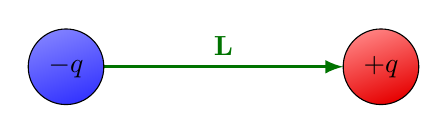
\begin{tikzpicture}
  \def\R{0.48}
  \def\L{4.0}
  \coordinate (Q-) at ( 0,0);
  \coordinate (Q+) at (\L,0);
  \draw[vector]  (Q-) ++ (\R,0) --++ (\L-2*\R,0) node[midway,above] {$\mathbf{L}$};
  \draw[charge-] (Q-) circle (\R) node[scale=1.0] {$-q$};
  \draw[charge+] (Q+) circle (\R) node[scale=1.0] {$+q$};
\end{tikzpicture}


%% DIPOLE
%\begin{tikzpicture}
%  \def\R{0.48}
%  \def\a{2.0}
%  \coordinate (Q-) at (-\a,0);
%  \coordinate (Q+) at (+\a,0);
%  \coordinate (P)  at (+2.5*\a,0);
%  
%  \draw[->,thick] (-1.5*\a,0) -- (+3.0*\a,0); %node[right] {$x$};
%  \draw[thick] (0,0.1) -- (0,-0.1) node[below] {0};
%  \draw[vector,line width=2]  (Q-) ++ (\R,0) --++ ({2*(\a-\R)},0) node[midway,above] {$\mathbf{L}$};
%  \draw[charge-] (Q-) circle (\R) node[scale=1.0] {$-q$};
%  \draw[charge+] (Q+) circle (\R) node[scale=1.0] {$+q$};
%  \fill (P) circle (0.1) node[above=2] {P};
%  \node[below=12] at (Q-) {$-a$};
%  \node[below=12] at (Q+) {$+a$};
%  \node[below= 4] at (P)  {$x$};
%  
%\end{tikzpicture}


% DIPOLE - axis beneath
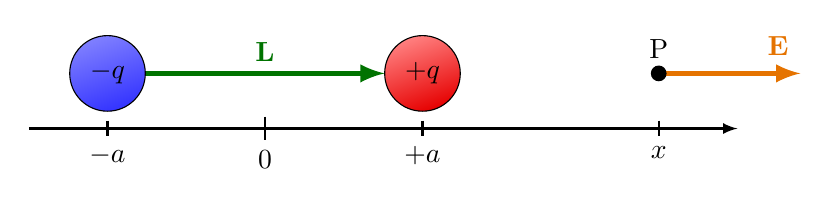
\begin{tikzpicture}
  \def\R{0.48}
  \def\a{2.0}
  \def\h{0.7}
  \coordinate (Q-) at (-\a,\h);
  \coordinate (Q+) at (+\a,\h);
  \coordinate (P)  at (+2.5*\a,\h);
  
  \draw[->,thick] (-1.5*\a,0) -- (+3.0*\a,0);
  \draw[thick] ( 0,0.15) --++ (0,-0.3) node[below] {0};
  \draw[thick] (-\a,0.1) --++ (0,-0.2) node[below] {$-a$};
  \draw[thick] (+\a,0.1) --++ (0,-0.2) node[below] {$+a$};
  \draw[thick] (2.5*\a,0.1) --++ (0,-0.2) node[below] {$x$};
  
  \draw[vector,line width=2]  (Q-) ++ (\R,0) --++ ({2*(\a-\R)},0) node[midway,above] {$\vb{L}$};
  \draw[charge-] (Q-) circle (\R) node[scale=1.0] {$-q$};
  \draw[charge+] (Q+) circle (\R) node[scale=1.0] {$+q$};
  \draw[vector,line width=2,Ecol] (P) --++ (0.9*\a,0) node[above=2,above left=0] {$\vb{E}$};
  \fill (P) circle (0.1) node[above=2] {P}; % node[below=2] {$x$};
  
\end{tikzpicture}


% DIPOLE in a uniform electric field
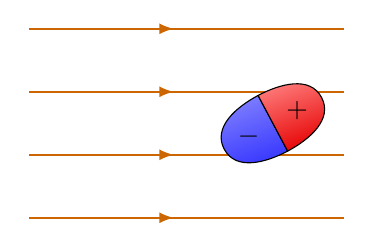
\begin{tikzpicture}
  \def\M{4}
  \def\xmax{2.0}
  \def\ymax{2.0}
  \def\a{0.7}
  \def\b{0.4}
  \def\ang{28}
  
  % ELECTRIC FIELD
  \foreach \i [evaluate={\y=-\ymax+2*\i*\ymax/(\M+1);}] in {1,...,\M}{
    \draw[EFieldLine=0.46] (-\xmax,\y) -- (\xmax,\y);
  }
  
  % DIPOLE
  \begin{scope}[shift={(1.1,0)},rotate=\ang]
    \draw[thick,charge-] (-\a,0) to[out=90,in=180] (0,\b) -- (0,-\b) to[out=180,in=-90] cycle;
    \draw[thick,charge+] ( \a,0) to[out=90,in=0] (0,\b) -- (0,-\b) to[out=0,in=-90] cycle;
    \node at (-\a/2,0) {$-$};
    \node at ( \a/2,0) {$+$};
  \end{scope}
  
\end{tikzpicture}


% DIPOLE in a non-uniform electric field
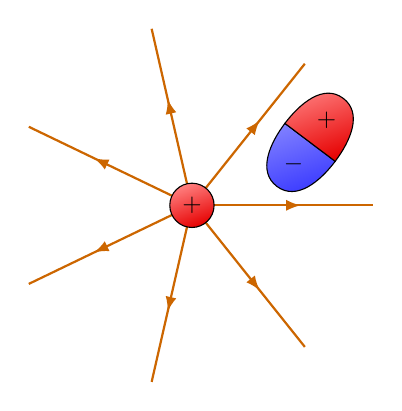
\begin{tikzpicture}
  \def\R{2.3}
  \def\a{0.7}
  \def\b{0.4}
  \def\angle{53}
  
  % FIELD
  \foreach \i [evaluate={\ang=\i*360/7;}] in {0,...,6}{
    \draw[EFieldLine={0.6}] (0,0) -- (\ang:\R);
  }
  \draw[charge+] (0,0) circle (8pt) node[black,scale=0.9] {$+$};
  
  % DIPOLE
  \begin{scope}[shift={(1.5,0.8)},rotate=\angle]
    \draw[thick,charge-] (-\a,0) to[out=90,in=180] (0,\b) -- (0,-\b) to[out=180,in=-90] cycle;
    \draw[thick,charge+] ( \a,0) to[out=90,in=0] (0,\b) -- (0,-\b) to[out=0,in=-90] cycle;
    \node[scale=0.9] at (-\a/2,0) {$-$};
    \node[scale=0.9] at ( \a/2,0) {$+$};
  \end{scope}
  
\end{tikzpicture}


% DIPOLE MOMENT in a uniform electric field
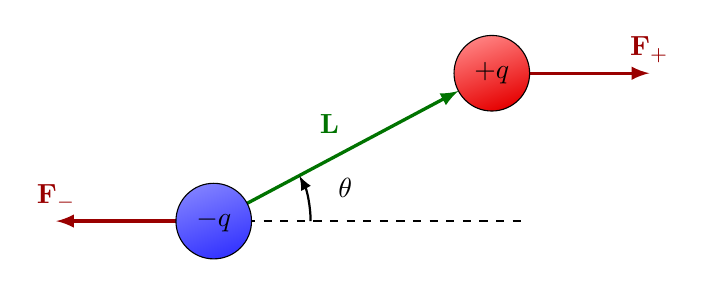
\begin{tikzpicture}
  \def\R{0.48}
  \def\L{4.0}
  \def\F{2.0}
  \def\ang{28}
  \coordinate (Q-) at ( 0,0);
  \coordinate (Q+) at (\ang:\L);
  \coordinate (X) at (\L,0);
  \draw[force] (Q-) --++ (-\F,0) node[above] {$\vb{F}_-$};
  \draw[force] (Q+) --++ (+\F,0) node[above] {$\vb{F}_+$};
  \draw[vector]  (Q-) ++(\ang:\R) --++ (\ang:\L-2*\R) node[midway,above left=1] {$\vb{L}$};
  \draw[dashed,thick] (Q-) -- (X);
  \draw pic[->,thick,"$\theta$",draw=black,angle radius=35,angle eccentricity=1.4]
    {angle = X--{Q-}--{Q+}};
  \draw[charge-] (Q-) circle (\R) node[scale=1.0] {$-q$};
  \draw[charge+] (Q+) circle (\R) node[scale=1.0] {$+q$};
\end{tikzpicture}


% DIPOLE MOMENT in a non-uniform electric field
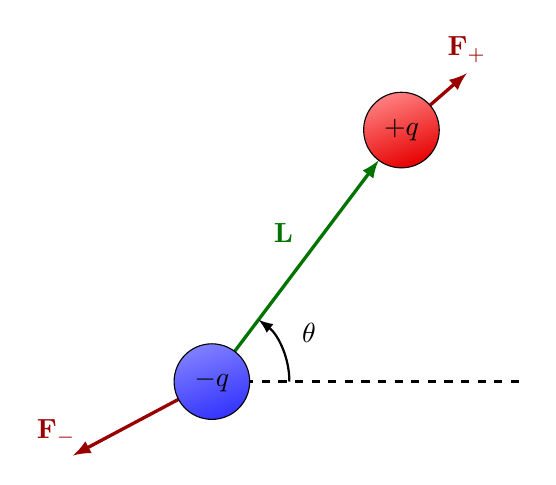
\begin{tikzpicture}
  \def\R{0.48}
  \def\L{4.0}
  \def\F{2.0}
  \def\ang{53}
  \coordinate (Q-) at ( 0,0);
  \coordinate (Q+) at (\ang:\L);
  \coordinate (X) at (\L,0);
  \draw[force] (Q-) --++ (155+\ang:\F) node[left=6,above] {$\vb{F}_-$};
  \draw[force] (Q+) --++ (\ang-12:0.55*\F) node[above] {$\vb{F}_+$};
  \draw[vector]  (Q-) ++(\ang:\R) --++ (\ang:\L-2*\R) node[midway,above left=1] {$\vb{L}$};
  \draw[dashed,thick] (Q-) -- (X);
  \draw pic[->,thick,"$\theta$",draw=black,angle radius=28,angle eccentricity=1.4]
    {angle = X--{Q-}--{Q+}};
  \draw[charge-] (Q-) circle (\R) node[scale=1.0] {$-q$};
  \draw[charge+] (Q+) circle (\R) node[scale=1.0] {$+q$};
\end{tikzpicture}


% WATER MOLECULE
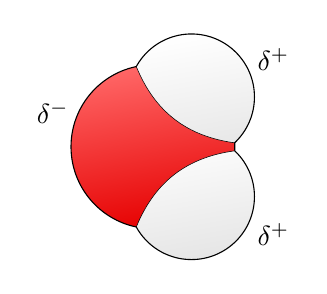
\begin{tikzpicture}[scale=0.8]
  \def\d{1.0}
  \def\RO{1.3}
  \def\RH{1.0}
  \def\ang{104.5}
  
  \coordinate (O)  at (  0, 0);
  \coordinate (H1) at ( \ang/2:\d);
  \coordinate (H2) at (-\ang/2:\d);
  \coordinate (T1) at ( \ang/2:{1.1*(\d+\RH)});
  \coordinate (T2) at (-\ang/2:{1.1*(\d+\RH)});
  
  \path[name path=O]  (O)  circle (\RO);
  \path[name path=H1] (H1) circle (\RH);
  \path[name path=H2] (H2) circle (\RH);
  
  \draw[O] (O) circle (\RO);
  
%  \path[name intersections={of=O and H1, name=i}];
%  %\draw (i-1) to [bend left] (i-2) to[out=140,in=-30,looseness=5] cycle;
%  %\draw (i-1) to [bend left] (i-2) to[controls=+(110:3*\RH) and +(0:3*\RH)] cycle;
%  %\draw (T1) -- (i-1) -- (i-2) -- cycle;
%  \draw (i-1) to[bend left] (i-2) to[out=180,in=120] (T1) to[out=0,in=-60] cycle;
%  %\draw[rotate=60] (i-1) --++ (0,\RH) --++ (0,+\RH) -- (i-2);
%  \path[name intersections={of=O and H2, name=i}];
%  %\draw (i-1) to [bend left] (i-2) to[out=0,in=-110,looseness=5] cycle;
%  \draw (i-1) to[bend left] (i-2) to[out=60,in=0] (T2) to[out=-120,in=180] cycle;
%  \draw (i-1) to [bend left] (i-2) --++ (150:0.1*\RH) --++ (60:1.2*\RH) --++ (-30:2.2*\RH) --++  (-120:1.2*\RH) -- cycle;
  
  \begin{scope}
    \path[name intersections={of=O and H1, name=i}];
    \clip (H1) circle (1.1*\RH);
    \clip (i-1) to[bend left] (i-2) to[out=180,in=\ang] (T1) to[out=0,in=-\ang/2] cycle;
    \draw[H] (H1) circle (\RH);
  \end{scope}
  \draw[very thin] (i-1) to [bend left] (i-2);
  
  \begin{scope}
    \path[name intersections={of=O and H2, name=i}];
    \clip (H2) circle (1.1*\RH);
    \clip (i-1) to[bend left] (i-2) to[out=\ang/2,in=0] (T2) to[out=-\ang,in=180] cycle;
    \draw[H] (H2) circle (\RH);
  \end{scope}
  \draw[very thin] (i-1) to [bend left] (i-2);
  
  %\node[scale=1.1]   at (      180:0.3*\RO) {O};
  %\node[scale=1.1]   at ( \ang/2:1.2*\d)  {H};
  %\node[scale=1.1]   at (-\ang/2:1.2*\d)  {H};
  \node[above left]  at (170:0.92*\RO)        {$\delta^-$};
  \node[above right] at ( 35:{0.92*(\d+\RH)}) {$\delta^+$};
  \node[below right] at (-35:{0.92*(\d+\RH)}) {$\delta^+$};
  
\end{tikzpicture}



\end{document}